\chapter{Proposed Training-Free Adaptive Control Approach}\label{ch:proposed}

\section{Introduction}\label{sec:prop-intro}
This chapter presents the two controllers proposed in this thesis. Both are small, rule-based programs that run beside a frozen detector and a frozen tracker, use only information that is available at run time, and need no training and no labels. Section~\ref{sec:acmot} presents the scene-adaptive controller of the detector operating point, AC-MOT, and Section~\ref{sec:ac-dev} explains how optimization experiments on calibration data led to its frozen values. Section~\ref{sec:scl} presents the self-calibrating control layer, SCL, which adapts the input and thresholds of the tracker to the detector's score distribution, and Section~\ref{sec:scl-dev} describes its development and freeze. Section~\ref{sec:prop-summary} summarizes the chapter. The evaluation of both controllers is given in Chapter~\ref{ch:results}.

\section{Scene-Adaptive Detector Operating-Point Controller (AC-MOT)}\label{sec:acmot}
AC-MOT is a small, rule-based controller that runs next to the detector. On frame 1 and then on every tenth frame, it measures cheap cues of the current image and of the boxes tracked in the previous frame (Section~\ref{sec:ac-cues}), averages the recent crowd level into a scene complexity index (SCI) (Section~\ref{sec:ac-sci}), chooses a target state (LOW, MEDIUM, or HIGH), adjusts it with a recovery probe and hysteresis and dwell rules (Section~\ref{sec:ac-states}), and maps the state to one of three fixed detector operating points (Section~\ref{sec:ac-actions}). Section~\ref{sec:ac-constants} explains how each value is chosen.

\subsection{Overview and Operating Point}\label{sec:ac-overview}
Figure~\ref{fig:ac-pipeline} shows where AC-MOT sits in the pipeline: the controller chooses the detector settings before the detector runs, and the detector and the tracker then run as usual. The detector settings at frame $t$ are called the operating point
\begin{equation}
\theta_t = (c_t, \eta_t, r_t),
\label{eq:ac-theta}
\end{equation}
which has three parts:
\begin{itemize}
\item $r_t$ is the input resolution, the long side of the resized image in pixels. A larger input shows small objects better but takes more time.
\item $\eta_t$ is the NMS IoU threshold. When two boxes overlap with an intersection over union (IoU) above $\eta_t$, the box with the lower score is removed. A lower $\eta_t$ removes more overlapping boxes.
\item $c_t$ is the score threshold. Boxes with a detector score below $c_t$ are removed before they reach the tracker. A higher $c_t$ passes fewer but more reliable boxes.
\end{itemize}
The detector weights and the tracker are frozen; AC-MOT changes only $\theta_t$.

The controller uses only information that is available at run time:
\begin{equation}
\theta_t = \pi\left(I_t, \mathcal{B}_{1:t-1}\right),
\label{eq:ac-policy}
\end{equation}
where $\pi$ is the control rule described in this section, $I_t$ is the image of the current frame, and $\mathcal{B}_{1:t-1}$ are the boxes that the tracker reported for the earlier frames $1$ to $t-1$. The tracker output of frame $t$ is used only from frame $t+1$ on. No ground truth, no future frame, and no detector score enters the decision.

\begin{figure}[tbp]
\centering
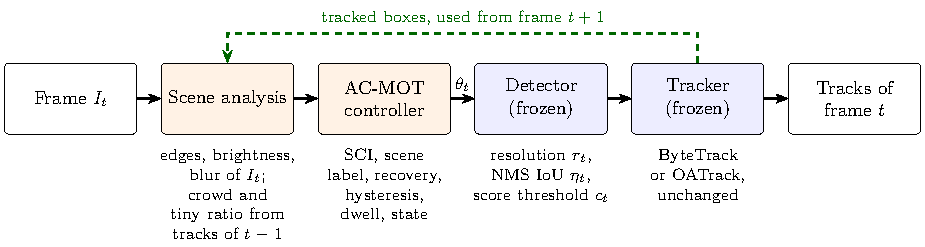
\includegraphics[width=0.98\textwidth]{figures/acmot_pipeline.pdf}
\caption{AC-MOT in a tracking-by-detection pipeline. Scene analysis and the controller choose the operating point $\theta_t=(c_t,\eta_t,r_t)$ before the detector runs. The frozen detector and tracker are not modified. Tracked boxes of frame $t$ feed the scene analysis of later frames (dashed arrow).}
\label{fig:ac-pipeline}
\end{figure}

\subsection{Scene Cues}\label{sec:ac-cues}
The controller needs a cheap description of the scene. Scene analysis therefore does not run on every frame. It runs on frame 1 and then once every 10 frames ($t=1$ or $t \bmod 10 = 1$, that is, frames 1, 11, 21, \dots). Each of these frames is an analysis step $j$. Between two analysis steps the controller keeps its last decision. Two kinds of cues are computed at each step: image cues, which describe how the current frame looks, and box cues, which describe the objects that the tracker found in the previous frame.

\emph{Image cues of the current frame.} The frame is reduced to a quarter of its width and height and converted to gray levels, so that the cues are cheap to compute. Three cues are then measured:
\begin{itemize}
\item the edge density $e_t$, the fraction of pixels marked as edges by the Canny detector (lower and upper thresholds 50 and 120); many edges indicate a cluttered scene;
\item the brightness $\beta_t$, the mean gray level from 0 (black) to 255 (white); a low value indicates a dark or night scene;
\item the sharpness $\nu_t$, the variance of the Laplacian of the gray image \cite{pechpacheco2000blur}; a low value indicates a blurred frame.
\end{itemize}

\emph{Box cues of the previous frame.} Let $N_j$ be the number of boxes that the tracker reported for frame $t-1$, and let $a_i$ be the area of box $i$ in pixels of the original image. The crowd cue and the tiny-object ratio are
\begin{align}
C_j&=\min\!\left(\frac{N_j}{30},1\right),\label{eq:ac-crowd}\\
T_j&=\frac{1}{N_j}\sum_{i=1}^{N_j}\mathbf{1}\!\left[a_i<32^2\right].\label{eq:ac-tiny}
\end{align}
$C_j$ is the number of tracked objects divided by 30 and capped at 1, so every frame with 30 or more objects has $C_j=1$. $T_j$ is the fraction of tracked boxes smaller than $32\times32$ pixels, which is the size limit of small objects in the COCO benchmark \cite{lin2014coco}. The indicator $\mathbf{1}[\cdot]$ is 1 when its condition holds and 0 otherwise, and $T_j=0$ when $N_j=0$.

\subsection{Scene Complexity Index and Scene Label}\label{sec:ac-sci}
The SCI measures how crowded the recent frames are. A single frame is a noisy measurement, because the tracker may miss or add a few objects in any frame, so the SCI averages over time. It is the mean crowd cue of the last seven analysis steps:
\begin{equation}
S_j=\frac{1}{|H_j|}\sum_{k\in H_j} C_k,
\label{eq:ac-sci}
\end{equation}
where $H_j$ holds the steps $j-6,\dots,j$ (fewer at the start of a video) and $|H_j|$ is their number. With a stride of 10 frames, the seven steps cover about the last 60 frames, so a single unusual frame changes $S_j$ only a little. Because $C_j\le1$, $S_j$ lies between 0 and 1.

The SCI uses the crowd cue alone, selected by the cue audit of Section~\ref{sec:ac-modern}. The other four cues are still used as checks on the state, mainly through the scene label
\begin{equation}
\ell_j=\begin{cases}
\text{night}   & \text{if } \beta_t<80,\\
\text{blur}    & \text{else if } \nu_t<180,\\
\text{tiny}    & \text{else if } T_j>0.50,\\
\text{crowded} & \text{else if } C_j>0.65 \text{ or } e_t>0.13,\\
\text{clear}   & \text{otherwise.}
\end{cases}
\label{eq:ac-label}
\end{equation}
The conditions are checked from top to bottom, and the first one that holds gives the label. For example, $T_j>0.50$ means that more than half of the tracked boxes are tiny, and $C_j>0.65$ means that at least 20 objects are tracked.

Only the crowd cue enters the SCI, and it also enters the crowded label. The tiny-object ratio $T_j$ is used by the state rules of Section~\ref{sec:ac-states} and gives the tiny label, and the edge density $e_t$ is used only through the crowded label. The brightness $\beta_t$ and the sharpness $\nu_t$ act only through the night and blur labels, which do not lead to MEDIUM or HIGH by themselves: because they are checked first, a dark or blurred frame cannot receive the crowded or tiny label, while the SCI conditions and the tiny-object guard of Eq.~\eqref{eq:ac-target} still apply.

\subsection{Three-State Controller}\label{sec:ac-states}
The controller is always in one of three states: LOW, MEDIUM, or HIGH. The names describe the scene: LOW for a sparse scene, HIGH for a crowded scene or a scene of mostly tiny objects. They do not rank the input size: in the final action map the HIGH state uses the smallest input (Table~\ref{tab:ac-actions}). The state is updated only at analysis steps, in four steps (Algorithm~\ref{alg:ac-controller}). Step~1 proposes a target state from the cues. Steps~2--4 adjust this target so that the controller reacts to a sudden drop in the object count but does not switch back and forth.

\emph{Step 1: target state.} The target is the state that the current cues ask for. It is given by the SCI, the tiny-object ratio, and the scene label:
\begin{equation}
g_j=\begin{cases}
\text{HIGH}   & \text{if } S_j>\tau_h \text{ or } T_j>0.50,\\
\text{MEDIUM} & \text{else if } S_j>\tau_m \text{ or } \ell_j\in\{\text{crowded},\text{tiny}\},\\
\text{LOW}    & \text{otherwise,}
\end{cases}
\label{eq:ac-target}
\end{equation}
where $\tau_m=0.297$ and $\tau_h=0.511$ are the two SCI thresholds (Table~\ref{tab:ac-constants}). Since $S_j$ is the recent average number of tracked objects divided by 30, the SCI conditions give MEDIUM above about 9 objects ($30\tau_m=8.9$) and HIGH above about 15 objects ($30\tau_h=15.3$).

\emph{Step 2: recovery probe.} The SCI averages seven steps, so it reacts slowly when the tracker suddenly reports far fewer objects than a few steps earlier. The recovery probe responds to such a collapse of the object count. Instead of letting the falling count move the controller toward a lower state, it sets the target to HIGH for a short time. To detect a collapse, it keeps a slowly decaying peak $P_j$ of the object count and a drop counter $d_j$:
\begin{align}
d_j&=\begin{cases}
d_{j-1}+1 & \text{if } P_{j-1}\ge5 \text{ and } N_j<0.40\,P_{j-1},\\
0         & \text{otherwise,}
\end{cases}\label{eq:ac-drop}\\
P_j&=\max\left(N_j,\lfloor 0.8\,P_{j-1}\rfloor\right),\label{eq:ac-peak}
\end{align}
with $P_0=d_0=0$. A collapse is detected when at least 5 objects have been seen before and fewer than 40\% of them remain. The peak loses 20\% at each step, so an old peak is forgotten after a few steps. While $1\le d_j\le3$, the target $g_j$ is set to HIGH, so the probe lasts at most three analysis steps (30 frames); the dwell rule of Step~4 still applies.

\emph{Step 3: hysteresis.} Without a margin, a scene whose SCI stays close to a threshold would make the controller switch at almost every step. Hysteresis prevents this: a move to a lower state is held while the scene is still close to difficult:
\begin{equation}
g_j\leftarrow\begin{cases}
\text{HIGH}   & \text{if } q_{j-1}=\text{HIGH} \text{ and } (S_j>0.50 \text{ or } T_j>0.40),\\
\text{MEDIUM} & \text{if } q_{j-1}=\text{MEDIUM},\ g_j=\text{LOW} \text{ and } S_j>0.25,\\
g_j           & \text{otherwise.}
\end{cases}
\label{eq:ac-hold}
\end{equation}
The hold values lie just below the values that lead into each state ($0.50<\tau_h$, 0.40 below the tiny guard of 0.50, and $0.25<\tau_m$). Upward moves are not held.

\emph{Step 4: dwell.} The dwell rule sets a minimum time between two changes. After a change, the state is kept for at least 30 frames, that is, three analysis steps:
\begin{equation}
q_j=\begin{cases}
g_j     & \text{if } t-t_c\ge30,\\
q_{j-1} & \text{otherwise,}
\end{cases}
\label{eq:ac-dwell}
\end{equation}
where $t_c$ is the frame of the last state change. The controller starts in LOW with $t_c=1$, so the first change is possible at frame 31. Whenever $q_j\ne q_{j-1}$, $t_c$ is set to $t$.

\emph{Why changes are kept rare.} Each change of state changes the boxes that reach the tracker, so the temporal rules let the state follow lasting changes of the scene, not single frames: the seven-step window smooths the SCI over about 60 frames, the holds add a margin below each threshold, and the dwell rule allows at most one change every 30 frames.

\emph{Example.} Consider a clear, sharp video in which the tracker reports 20 objects of normal size in every frame ($C_j=0.67$), and only 10 objects from frame 71 on. The controller starts in LOW. The first step sees no earlier boxes ($C_j=0$), so $S_j$ grows as the window fills: 0.33 at frame 11, 0.44 at frame 21, and 0.50 at frame 31. The target is MEDIUM from frame 11, but the dwell rule keeps LOW until frame 31, where the state becomes MEDIUM. From frame 41, $S_j$ exceeds $\tau_h$ and the target is HIGH; the dwell rule delays this change to frame 61. When the scene thins, $S_j$ falls slowly because the window still holds the earlier steps, so the state stays HIGH until frame 101. At frame 111, $S_j=0.48$ is below both $\tau_h$ and the hold value of 0.50, and the state returns to MEDIUM. It then stays in MEDIUM, because 10 tracked objects keep $S_j$ at about 0.33, above $\tau_m$.

The state $q_j$ then selects the operating point from the action map, and the detector uses it until the next analysis step.

\begin{algorithm}[tbp]
\caption{AC-MOT controller for one video.}\label{alg:ac-controller}
\begin{algorithmic}[1]
\Require frames $I_1, I_2, \dots$; frozen detector and tracker; constants of Table~\ref{tab:ac-constants}
\Ensure tracks of every frame
\State $j\gets0$; $q_0\gets$ LOW; $P_0\gets0$; $d_0\gets0$; $t_c\gets1$
\For{each frame $t=1,2,\dots$}
  \If{$t=1$ \textbf{or} $t \bmod 10=1$} \Comment{analysis step, every 10 frames}
    \State $j\gets j+1$
    \State $e_t,\beta_t,\nu_t\gets$ image cues of $I_t$ \Comment{Section~\ref{sec:ac-cues}}
    \State $N_j,C_j,T_j\gets$ cues of the tracked boxes of frame $t-1$ \Comment{no boxes at $t=1$}
    \State $S_j\gets$ mean of $C_k$ over the last seven steps $k\in H_j$ \Comment{SCI, Eq.~\eqref{eq:ac-sci}}
    \State $\ell_j\gets$ label, Eq.~\eqref{eq:ac-label}; $g_j\gets$ target, Eq.~\eqref{eq:ac-target} \Comment{Step 1: target}
    \State update $d_j$ and $P_j$, Eqs.~\eqref{eq:ac-drop}--\eqref{eq:ac-peak}
    \If{$1\leq d_j\leq3$} $g_j\gets$ HIGH \Comment{Step 2: recovery probe}
    \EndIf
    \State apply hysteresis to $g_j$, Eq.~\eqref{eq:ac-hold} \Comment{Step 3: hysteresis}
    \If{$t-t_c\geq30$ \textbf{and} $g_j\neq q_{j-1}$} \Comment{Step 4: dwell}
      \State $q_j\gets g_j$; $t_c\gets t$
    \Else
      \State $q_j\gets q_{j-1}$
    \EndIf
  \EndIf
  \State $(r_t,\eta_t,c_t)\gets$ action of state $q_j$, Table~\ref{tab:ac-actions} \Comment{kept until the next analysis step}
  \State detect with $r_t$ and $\eta_t$; drop boxes with score $<c_t$
  \State update the tracker; store its boxes of frame $t$ \Comment{used from frame $t+1$}
\EndFor
\end{algorithmic}
\end{algorithm}

\subsection{Action Map}\label{sec:ac-actions}
Table~\ref{tab:ac-actions} gives the operating point of each state. The actions are not set by hand: they are selected together with $\tau_m$ and $\tau_h$ by the joint search on the calibration sequences, whose objective is the change in HOTA, a metric that balances detection and association (Section~\ref{sec:ac-constants}).

In LOW, the sparse state, the detector uses the largest input, loose NMS, and a low score threshold, so it passes more weak boxes. In MEDIUM and HIGH it passes only boxes with a score of at least 0.40. The HIGH state, used for crowded scenes and for scenes of mostly tiny objects, thus has the smallest input. This may look surprising, since a larger input shows small objects better, but the search optimizes tracking quality, not the detection of every small object: a score threshold of 0.40 gives the tracker fewer but more reliable boxes (Section~\ref{sec:ac-modern}), and the smaller input costs less detector time. Chapter~\ref{ch:results} shows that the main effect of AC-MOT is a more selective detection stream: fewer false positives and identity switches, with similar or slightly lower recall. This action is the result of the search, not a general rule that crowded scenes need smaller inputs.

The score threshold $c_t$ is applied on the detector side before the tracker. It is separate from any confidence gate inside the tracker, such as the fixed tracker-side gate of OATrack.

\begin{table}[tbp]
\centering
\caption{Action map of AC-MOT. State names describe scene difficulty, not a resolution rank. Selected by the joint search on the calibration sequences.}
\label{tab:ac-actions}
\begin{tabular}{lrrr}
\toprule
State & Resolution $r$ (pixels) & NMS IoU $\eta$ & Score threshold $c$\\
\midrule
LOW & 1536 & 0.70 & 0.10\\
MEDIUM & 1280 & 0.45 & 0.40\\
HIGH & 1088 & 0.60 & 0.40\\
\bottomrule
\end{tabular}
\end{table}

\subsection{Selection of Parameter Values}\label{sec:ac-constants}
All values of Tables~\ref{tab:ac-actions} and~\ref{tab:ac-constants} are fixed before the final evaluation and are not changed after it. The last column of Table~\ref{tab:ac-constants} gives the source of each value. There are four sources.

\emph{Joint search on the calibration sequences.} The SCI thresholds $\tau_m$ and $\tau_h$ and the action map are selected together by an Optuna TPE search with 60 trials \cite{akiba2019optuna}; the search ranges are given in Section~\ref{sec:ac-modern}. The calibration sequences are eight sequences of the VisDrone2019-MOT training split. They serve as the validation (tuning) data of the final stage and are disjoint from the evaluation sequences. Each trial is scored by four-fold cross-validation (CV), with two sequences held out in each fold, as the mean change in HOTA against the baseline. The candidate values come from existing settings. The input sizes (1088, 1280, and 1536 pixels) and NMS values (0.45, 0.60, and 0.70) are the operating points for which detector outputs are cached; 1536 pixels with NMS 0.70 is the baseline point, and 0.70 is the default NMS value of the Ultralytics detector. The three score thresholds are the low and high thresholds of ByteTrack (0.10 and 0.25) and the confidence gate of OATrack (0.40).

\emph{Cue audit on the calibration sequences.} The choice of the crowd cue as the only SCI input comes from testing all 31 non-empty subsets of the five cues with the same cross-validation (Section~\ref{sec:ac-modern}).

\emph{Temporal sweep on the validation split.} The analysis stride and the SCI window are selected in the first development stage, with the YOLOv8n pipeline, on the VisDrone2019-MOT validation sequences. The sweep tests 25 combinations: windows of 1, 3, 5, 7, and 9 analysis steps and strides of 1, 5, 10, 15, and 20 frames. Five of the 25 settings meet both constraints of that stage, at least 25 frames per second (FPS) and at most 271 identity switches (the number of the original controller on the same data). Among them, a window of 7 and a stride of 10 give the highest MOTA, 18.165 against 18.044 for the next setting. Operating-point sweeps on the same data cover input resolutions from 512 to 960 pixels, confidence thresholds from 0.05 to 0.50, and NMS thresholds from 0.30 to 0.80, and define the supported values of the first optimized profiles (Section~\ref{sec:ac-dev}).

\emph{Fixed design values.} The tiny-object area follows the COCO definition of small objects \cite{lin2014coco}. The remaining values (the crowd normalizer, the Canny thresholds, the label thresholds, the recovery, hold, and dwell values, and the initial state) come from the original AC-MOT controller and are kept unchanged in every search of the final stage, so the searched values are matched to them. For example, the crowd normalizer of 30 only sets the scale of $S_j$: $\tau_m$ and $\tau_h$ are searched on this scale and correspond to about 9 and 15 tracked objects.

\begin{table}[tbp]
\centering
\caption{Values of the AC-MOT controller and how each value is chosen. Calibration sequences: eight VisDrone2019-MOT training sequences used as tuning data, disjoint from the evaluation sequences. CV: four-fold cross-validation.}
\label{tab:ac-constants}
\begin{tabular}{>{\raggedright\arraybackslash}p{1.6cm}>{\raggedright\arraybackslash}p{4.6cm}>{\raggedright\arraybackslash}p{2.6cm}>{\raggedright\arraybackslash}p{5.6cm}}
\toprule
Symbol & Meaning & Value & How the value is chosen\\
\midrule
$\tau_m$ & SCI threshold for MEDIUM, Eq.~\eqref{eq:ac-target} & 0.297 & joint TPE search on the calibration sequences, 60 trials, CV\\
$\tau_h$ & SCI threshold for HIGH, Eq.~\eqref{eq:ac-target} & 0.511 & same joint search\\
$(r,\eta,c)$ & operating point of each state & Table~\ref{tab:ac-actions} & same joint search over $\{1088,1280,1536\}\times\{0.45,0.60,0.70\}\times\{0.10,0.25,0.40\}$\\
-- & SCI input cue & crowd only & cue audit of all 31 cue subsets on the calibration sequences, CV\\
-- & analysis stride & 10 frames & temporal sweep of 25 settings on the validation split; highest MOTA with $\geq$25 FPS and $\leq$271 IDS\\
$|H_j|$ & SCI window & 7 steps & same temporal sweep\\
-- & tiny-object area & $32\times32$ pixels & COCO small-object limit \cite{lin2014coco}\\
-- & crowd normalizer, Eq.~\eqref{eq:ac-crowd} & 30 boxes & original controller; sets the scale on which $\tau_m$, $\tau_h$ are searched\\
-- & Canny thresholds (lower, upper) & 50, 120 & original controller; fixed in all final-stage searches\\
-- & night and blur labels, Eq.~\eqref{eq:ac-label} & $\beta_t<80$, $\nu_t<180$ & original controller; fixed in all final-stage searches\\
-- & crowded label, Eq.~\eqref{eq:ac-label} & $C_j>0.65$ or $e_t>0.13$ & original controller; fixed in all final-stage searches\\
-- & tiny label and HIGH guard, Eqs.~\eqref{eq:ac-label}, \eqref{eq:ac-target} & $T_j>0.50$ & original controller; fixed in all final-stage searches\\
-- & recovery: minimum peak, drop ratio, peak decay, steps & 5, 0.40, 0.80, 3 & original controller; fixed in all final-stage searches\\
-- & holds in HIGH ($S_j$, $T_j$) and MEDIUM ($S_j$), Eq.~\eqref{eq:ac-hold} & (0.50, 0.40), 0.25 & original controller; fixed in all final-stage searches\\
-- & dwell, Eq.~\eqref{eq:ac-dwell} & 30 frames & original controller; fixed in all final-stage searches\\
-- & initial state & LOW & original controller; fixed in all final-stage searches\\
\bottomrule
\end{tabular}
\end{table}

\section{Development of the AC-MOT Controller}\label{sec:ac-dev}
The controller of Section~\ref{sec:acmot} is the result of four development stages. The quality-oriented profile (Section~\ref{sec:ac-quality}) asked whether a scene index that steers the detector settings can beat a fixed default; the identity-aware profile (Section~\ref{sec:ac-identity}) made identity stability and speed explicit objectives; the transfer studies (Section~\ref{sec:ac-transfer}) tested other data and pipelines; and the modern stage (Section~\ref{sec:ac-modern}) built the frozen controller for a modern detector with separate calibration data. The first three stages are historical: they used a weighted five-cue index with interpolated confidence and NMS values and three resolution levels (the SparseTrack study used a single edge-driven NMS rule), other detectors, and other evaluation protocols. Their numbers are reported in their own tables, each against its own baseline, and are not pooled with the modern results.

\subsection{Quality-Oriented Profile}\label{sec:ac-quality}
\emph{Baseline.} The reference pipeline is the pretrained YOLOv8n detector \cite{jocher2023yolov8} followed by ByteTrack \cite{zhang2022bytetrack}, both at their default settings: confidence threshold 0.25, NMS IoU threshold 0.45, input size 640 pixels, and the default ByteTrack parameters listed in Section~\ref{sec:res-env}. It runs with one fixed operating point for the whole video.

\emph{Method.} The first optimization-derived profile kept the same detector, used a tuned ByteTrack profile, and searched only on the VisDrone2019-MOT validation split. Each of five cues was normalized with validation statistics, and the index was their weighted sum
\begin{equation}
S_j=\sum_{k\in\{c,t,e,n,b\}}w_k\,x_{k,j},
\label{eq:ac-histsci}
\end{equation}
where $k$ runs over the cues (c: crowd count, t: fraction of earlier boxes below $32\times32$ pixels, e: edge density, n: low brightness, b: low Laplacian variance), $x_{k,j}$ is the normalized value of cue $k$ at analysis step $j$, and $w_k$ is its weight, with $w_k\geq0$ and $\sum_k w_k=1$. The index was averaged over seven analyses taken every ten frames. Confidence and NMS were interpolated linearly between the values at $S=0$ and $S=1$, and two sorted thresholds selected one of three resolutions (512, 928, 960 pixels).

An Optuna TPE study \cite{akiba2019optuna} jointly searched the five weights, the confidence and NMS end points, and the two thresholds. The resolution levels, the supported confidence values $\{0.25,\dots,0.45\}$, the supported NMS values from 0.30 to 0.70, and the temporal settings were fixed beforehand by validation sweeps (Section~\ref{sec:ac-constants}). The selection rule kept trials with at least 25 FPS and at most 271 IDS (the IDS of the original controller on the same validation data) and then took the highest MOTA, with lower IDS, HOTA, IDF1, and FPS as tie-breaks. The frozen profile (archived as Trial~24) has $w_c=0.1294928$, $w_t=0.2217477$, $w_e=0.4337134$, $w_n=0.0535577$, $w_b=0.1614885$, confidence end points $(0.30,0.40)$, NMS end points $(0.35,0.35)$, and thresholds $(0.1353494, 0.2872868)$. On validation it reached MOTA 23.038, HOTA 36.110, IDF1 40.758, and IDS 270 at 37.169 FPS.

\emph{Comparison.} Table~\ref{tab:ac-quality} compares the profile with the baseline on the historical VisDrone test-dev split, with paired bootstrap intervals (5000 resamples, seed 42). A scene index that steers the detector settings improved tracking quality over the fixed default point, with HOTA, MOTA, and IDF1 intervals above zero. The IDS interval, $[-114, 219]$, includes zero; the next stage made identity stability an explicit objective. The final controller keeps two parts of this stage: the stride of 10 frames and the window of seven steps from its temporal sweep (Section~\ref{sec:ac-constants}), and the five kinds of scene cues, which were audited again in the modern stage.

\begin{table}[tbp]
\centering
\caption{Quality-oriented profile versus its baseline (YOLOv8n with ByteTrack at default settings) on VisDrone test-dev, historical protocol. Gain: paired bootstrap difference with 95\% interval; for IDS it is the reduction.}
\label{tab:ac-quality}
\begin{tabular}{lrrl}
\toprule
Metric & Baseline & Quality & Gain [95\% CI]\\
\midrule
HOTA & 28.430 & 33.835 & $+5.4051$ [$4.1273$, $6.9022$]\\
MOTA & 19.729 & 26.948 & $+7.2195$ [$5.4362$, $9.2934$]\\
IDF1 & 32.724 & 41.546 & $+8.8220$ [$6.9005$, $11.0537$]\\
IDS & 1235 & 1184 & $51$ [$-114$, $219$]\\
FPS & 36.528 & 38.985 & --\\
\bottomrule
\end{tabular}
\end{table}

\subsection{Identity-Aware Pareto Profile}\label{sec:ac-identity}
\emph{Baseline.} The baseline is the same YOLOv8n and ByteTrack pipeline at default settings (Section~\ref{sec:ac-quality}).

\emph{Method.} The second study kept the same cues, operating levels, temporal settings, and validation data, but changed the question. It maximized MOTA and minimized IDS subject only to $\mathrm{FPS}\geq25$, without the IDS gate. A seeded TPE sampler ran 49 completed trials. A trial dominated another when it had no lower MOTA and no higher IDS, with at least one strict improvement, and the feasible Pareto front was built from these relations. The balanced candidate maximized an equal-weight score of normalized MOTA and normalized IDS reduction, with HOTA, IDF1, FPS, and trial index as tie-breaks. The selected profile (archived as Trial~22) has weights $w_c=0.1646453$, $w_t=0.1746265$, $w_e=0.5076113$, $w_n=0.1206956$, $w_b=0.0324213$, confidence end points $(0.40,0.40)$, NMS end points $(0.60,0.35)$, and thresholds $(0.2927136, 0.6661672)$. On validation it reached MOTA 19.330, HOTA 31.651, IDF1 34.226, and IDS 168 at 51.406 FPS.

\emph{Comparison.} Table~\ref{tab:ac-identity} compares the profile with the baseline on test-dev. It removes 316 IDS and raises throughput from 36.528 to 46.024 FPS, while HOTA, MOTA, and IDF1 also rise. Against the quality-oriented profile it has 265 fewer IDS $[82, 502]$ and $-2.617$ HOTA $[-4.004, -1.694]$. The two profiles therefore answer different questions: one favors overall quality and the other favors identity stability and speed. The detector operating point controls a trade-off between quality, identity stability, and speed, and the objective of the search decides which side is favored.

\begin{table}[tbp]
\centering
\caption{Identity-aware profile versus its baseline (YOLOv8n with ByteTrack at default settings) on VisDrone test-dev, historical protocol. Gain: paired bootstrap difference with 95\% interval; for IDS it is the reduction.}
\label{tab:ac-identity}
\begin{tabular}{lrrl}
\toprule
Metric & Baseline & Identity & Gain [95\% CI]\\
\midrule
HOTA & 28.430 & 31.218 & $+2.788$ [$0.747$, $4.660$]\\
MOTA & 19.729 & 23.792 & $+4.063$ [$0.952$, $6.886$]\\
IDF1 & 32.724 & 37.870 & $+5.146$ [$2.028$, $8.080$]\\
IDS & 1235 & 919 & $316$ [$175$, $470$]\\
FPS & 36.528 & 46.024 & --\\
\bottomrule
\end{tabular}
\end{table}

\subsection{Transfer and Cross-Pipeline Studies}\label{sec:ac-transfer}
This stage applied the historical controllers outside their development setting: to a second dataset, and to two other detector--tracker pipelines.

\emph{UAVDT.} The baseline is again YOLOv8n with ByteTrack at default settings (Section~\ref{sec:ac-quality}). Both frozen profiles were applied to UAVDT \cite{du2018uavdt} without retuning (Table~\ref{tab:ac-histuavdt}). The quality-oriented profile raised HOTA by 4.305 points $[2.740, 5.709]$ and the identity-aware profile by 2.845 points $[1.238, 4.348]$; their IDS reductions are 237 $[104, 377]$ and 250 $[110, 404]$.

\begin{table}[tbp]
\centering
\caption{Historical UAVDT transfer without retuning. Baseline: YOLOv8n with ByteTrack at default settings.}
\label{tab:ac-histuavdt}
\begin{tabular}{lrrr}
\toprule
Metric & Baseline & Quality & Identity\\
\midrule
HOTA & 24.085 & 28.390 & 26.930\\
MOTA & 13.841 & 17.399 & 16.118\\
IDF1 & 27.887 & 34.453 & 32.014\\
IDS & 558 & 321 & 308\\
FPS & 65.015 & 58.353 & 61.462\\
\bottomrule
\end{tabular}
\end{table}

\emph{U2MOT on VisDrone.} The baseline is the published U2MOT tracker \cite{liu2023u2mot} with its released YOLOX-X detector, run at its own static setting. Seven VisDrone validation sequences served for development and 17 test-dev sequences for evaluation. The cue weights and transforms of the quality-oriented profile were kept, the tracker was not modified, and the action boundaries were set to the 33rd and 67th percentiles of the index on the U2MOT validation run, without using ground truth. Table~\ref{tab:ac-u2mot} (top) gives the comparison: the controlled pipeline has 87 fewer IDS and 1230 fewer false positives, while MOTA is almost unchanged and false negatives are higher.

\emph{SparseTrack on MOT17.} The baseline is the published SparseTrack tracker \cite{liu2025sparsetrack} with a fixed NMS IoU threshold of 0.75, on the seven MOT17 val-half sequences (2652 frames) \cite{dendorfer2021motchallenge}. A minimal edge-driven rule switched only the NMS threshold, between 0.70 and 0.80; its threshold came from a leave-one-sequence-out study on the same sequences. Table~\ref{tab:ac-u2mot} (bottom) gives the comparison: the adaptive rule reduces IDS from 136 to 123, with MOTA $+0.0371$ points $[-0.041, +0.182]$.

\begin{table}[tbp]
\centering
\caption{Cross-pipeline studies. Top: U2MOT with its YOLOX-X detector at its static setting on VisDrone test-dev. Bottom: SparseTrack with a fixed NMS IoU threshold of 0.75 on MOT17 val-half.}
\label{tab:ac-u2mot}
\begin{tabular}{llrr}
\toprule
Pipeline & Metric & Baseline & With control\\
\midrule
U2MOT & MOTA & 53.873 & 53.767\\
 & IDF1 & 69.775 & 69.849\\
 & IDS & 1239 & 1152\\
 & FP & 41385 & 40155\\
 & FN & 63241 & 64801\\
\midrule
SparseTrack & MOTA & 76.8881 & 76.9252\\
 & IDF1 & 81.4943 & 81.5299\\
 & IDS & 136 & 123\\
\bottomrule
\end{tabular}
\end{table}

The frozen profiles kept their direction on UAVDT without retuning, and with U2MOT and SparseTrack the control mainly reduced IDS, with small changes in MOTA. Together these studies show that the preferred profile depends on the objective (quality or identity) and on the tracker host. This motivated a modern stage with a stronger detector, explicit calibration data, and two tracker hosts.

\subsection{Development of the Frozen Controller}\label{sec:ac-modern}
The modern stage decided which cues enter the SCI, which operating points each state uses, and where the SCI thresholds lie.

\emph{Baseline.} The modern baseline is the YOLO11m detector \cite{jocher2024yolo11}, in a public version trained on VisDrone2019-DET \cite{zhu2022visdrone}, run at a fixed operating point of 1536 pixels and NMS IoU 0.70 with no extra score threshold. It feeds ByteTrack \cite{zhang2022bytetrack} during development and both ByteTrack and OATrack \cite{qi2026oatrack} in the final evaluation. A large fixed input is a common choice for small aerial objects when no adaptation is used.

\emph{Data and protocol.} Eight sequences of the VisDrone2019-MOT training split (3282 frames) were declared as calibration data. They are disjoint from the seven evaluation sequences. The searches used the same four folds, each holding out two calibration sequences. Detector outputs were cached for every resolution and NMS value; a score threshold applied to the cache was checked to reproduce direct inference exactly. The steps are described below in the order in which they were carried out.

\emph{Resolution and NMS maps.} Two exhaustive grid searches, archived as Stages 1 and 2, searched the state-to-resolution and state-to-NMS maps. At this point the action of a state contained only the input resolution and the NMS value.

\emph{Cue audit.} The next search, archived as Stage 3A, asked which cues should form the SCI. It searched all 31 non-empty subsets of the five cues and selected \{crowd\}, which defines the crowd-selected SCI of Eq.~\eqref{eq:ac-sci}. The other cues were kept as guard and auxiliary cues of the state logic (Section~\ref{sec:ac-sci}).

\emph{Score threshold.} A separate sweep then tested the score threshold. At 1088 pixels and NMS 0.45, a fixed score threshold of 0.40 raised pooled calibration HOTA by $+0.881$ over 0.01 and improved seven of the eight sequences. The score threshold was therefore added as the third action dimension.

\emph{Final joint search.} The final search then selected the thresholds and the three-part actions together. It used 60 TPE trials (seed 43) and searched $\tau_m\in[0.10,0.50]$, $\tau_h\in[\tau_m+0.05,\min(\tau_m+0.40,0.90)]$, and for each state a resolution in $\{1088,1280,1536\}$, an NMS value in $\{0.45,0.60,0.70\}$, and a score threshold in $\{0.10,0.25,0.40\}$. The objective was the cross-validated mean change in HOTA against the baseline, with ByteTrack as host. A candidate was eligible only if it really adapted within the video rather than acting as one fixed operating point: it had to realize at least two distinct actions, each on at least 10\% of calibration frames, and switch within sequences. The frozen policy is the eligible candidate whose three states use three different actions that together vary all three parts of the operating point (Table~\ref{tab:ac-actions}). On calibration data it used LOW, MEDIUM, and HIGH on 7.6\%, 10.1\%, and 82.3\% of frames, with 0.607 state changes per 100 frames on average.

\emph{Comparison.} Table~\ref{tab:ac-folds} compares the frozen policy with the baseline on each calibration fold. All four folds are positive, with a CV mean of $+2.447$ HOTA. After these steps the thresholds, cue subset, and action map were frozen. The final comparison on the evaluation sequences is given in Chapter~\ref{ch:results}.

\begin{table}[tbp]
\centering
\caption{Frozen AC-MOT policy versus the modern baseline (YOLO11m at 1536 pixels and NMS 0.70, ByteTrack) on the four calibration folds: change in HOTA.}
\label{tab:ac-folds}
\begin{tabular}{lrrrrr}
\toprule
 & Fold 1 & Fold 2 & Fold 3 & Fold 4 & Mean\\
\midrule
$\Delta$HOTA & $+0.592$ & $+4.164$ & $+2.029$ & $+3.004$ & $+2.447$\\
\bottomrule
\end{tabular}
\end{table}

\section{Self-Calibrating Control Layer (SCL)}\label{sec:scl}
AC-MOT adapts the detector to the scene, but it assumes that the detector's scores keep the scale for which the tracker was tuned. The second controller addresses this assumption. SCL is a small, rule-based layer that runs once per frame between the detector and the tracker (Fig.~\ref{fig:scl-arch}). It groups the scores of recent frames (Section~\ref{sec:scl-calib}), decides whether they are clean or noisy (Section~\ref{sec:scl-modes}), acts on this decision, and can pass a weak candidate that clearly continues a track (Section~\ref{sec:scl-rescue}). The detector and the tracker are never changed. The tracker that SCL serves is called the \emph{host}; it gives SCL four of its published settings, the host contract (Section~\ref{sec:scl-contract}).

\subsection{Overview}\label{sec:scl-overview}
In short, a detection travels through SCL as follows. Its score is turned into a logit and compared with two splits computed from the scores of the last 10 frames: below the first split it is background, between the splits uncertain, and above the second confident. If most recent foreground scores are confident, the stream is clean and the detection reaches the tracker with its own score. Otherwise the stream is noisy: a background detection is dropped, and the others get new scores that tell the tracker whether they may start a track or only continue one. A weak detection that lies on a track of the previous frame can still be passed on. The tracker then does its own matching as usual. Its score enters the statistics only after the decision for its frame.

\begin{figure}[tbp]
\centering
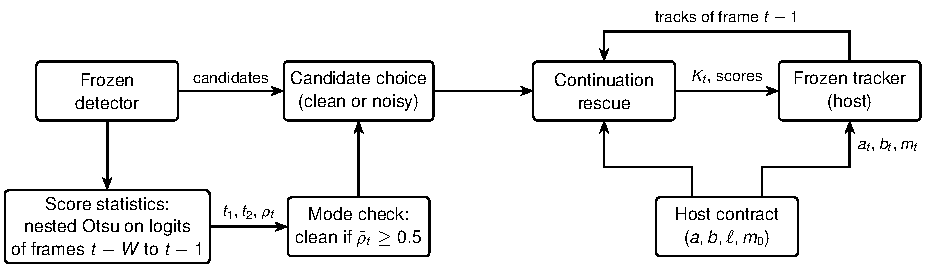
\includegraphics[width=0.98\textwidth]{figures/scl_architecture.pdf}
\caption{SCL between a frozen detector and a frozen tracker (the host). Boxes are processing steps and arrows show what each step passes on. The score statistics use earlier frames only. The host contract holds the tracker's published settings. The tracker receives the chosen candidates $K_t$, their scores, and its thresholds $a_t$, $b_t$ and tolerance $m_t$ for the frame.}
\label{fig:scl-arch}
\end{figure}

\subsection{Inputs and Outputs}\label{sec:scl-problem}
In each frame $t$, the detector gives candidates $D_t=\{(\mathbf{x}_i,s_i,c_i)\}$, each with a box $\mathbf{x}_i$, a score $s_i\in(0,1)$, and a class $c_i$. The layer works on the logit
\begin{equation}
z_i=\log\frac{s_i}{1-s_i},
\label{eq:scl-logit}
\end{equation}
the log-odds transformation of the confidence score. It converts a score between 0 and 1 into a value on an unrestricted scale while preserving the ordering of scores: a score of 0.5 gives $z_i=0$, 0.9 gives about $2.2$, and 0.1 about $-2.2$. The logistic function $\sigma(z)=1/(1+e^{-z})$ turns a logit back into a score. The layer uses logits for two reasons. Detector scores crowd near 0 and 1, where small differences in score are large differences in confidence; the logit spreads these regions out, so the histogram splits of Section~\ref{sec:scl-calib} separate the groups more clearly. And a common change of a detector's scores, a change of temperature, divides all logits by the same number, a simple stretch that the splits follow (Section~\ref{sec:scl-calib}).

The host gives its contract $h=(a,b,\ell,m_0)$: the score $a$ needed to match a track, the score $b$ needed to start one, the lowest score $\ell$ it uses, and its matching tolerance $m_0$, one minus the smallest IoU of two boxes that counts as a match. A single-stage tracker has $\ell=\min(a,b)$, a two-stage tracker $\ell<\min(a,b)$. In every frame the layer returns
\begin{equation}
\left(K_t,\tilde{s},a_t,b_t,m_t\right)=
\mathcal{L}\left(Z_{<t},D_t,\mathcal{T}_{t-1},g_t;\,h\right):
\label{eq:scl-layer}
\end{equation}
the candidates $K_t$ for the tracker, their scores, and its thresholds and tolerance, from the logits $Z_{<t}$ of earlier frames, the tracks $\mathcal{T}_{t-1}$, and a camera-motion measure $g_t$; no future frame is used.

\subsection{Self-Calibration from Detector Scores}\label{sec:scl-calib}
The layer collects the logits $Z_t^W$ of the candidates of the last $W=10$ frames and splits them twice with Otsu's method \cite{otsu1979} (Eq.~\eqref{eq:bg-otsu}). The first split, $t_1$, separates background (low logits) from foreground; the second, $t_2$, found on the foreground only, divides it into uncertain and confident candidates. The share of confident candidates in the foreground,
\begin{equation}
\rho_t=\frac{\left|\{z\in Z_t^W: z\ge t_2\}\right|}{\left|\{z\in Z_t^W: z\ge t_1\}\right|},
\label{eq:scl-rho}
\end{equation}
describes the shape of the score distribution and needs no labels: if 30 of 40 foreground candidates are confident, $\rho_t=0.75$. Otsu's method is used because it picks a split from the data alone, without labels or tuning, and applying it twice gives the three groups that one threshold cannot.

For example, for the scores 0.02, 0.03, 0.05, 0.4, 0.5, 0.9, and 0.95 (logits $-3.9$, $-3.5$, $-2.9$, $-0.4$, 0, 2.2, and 2.9), the first split separates the three lowest scores as background, and the second divides the other four into 0.4 and 0.5 (uncertain) and 0.9 and 0.95 (confident), so $\rho_t=2/4=0.5$. Because the splits are made on logits, they move with the scores when the whole logit scale is stretched or shifted, and each group keeps the same candidates. Figure~\ref{fig:scl-groups} shows the groups for a clean and a noisy stream. When a detector emits very few low scores, the first split falls inside the objects; since clutter usually gives more candidates than the objects do, a window with fewer candidates below $t_1$ than above it counts as clean, $\rho_t=1$ (background check).

\begin{figure}[tbp]
\centering
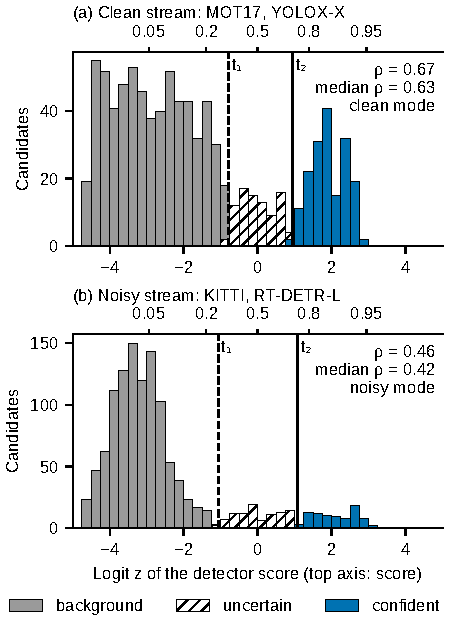
\includegraphics[width=0.62\textwidth]{figures/scl_score_groups.pdf}
\caption{What the layer sees: the logits of the candidates of the last 10 frames, just before its decision for frame 101, with the Otsu splits $t_1$ (dashed line) and $t_2$ (solid line). Plain light bars: background; hatched bars: uncertain; plain dark bars: confident. The top axis gives the matching detector score. (a) MOT17-02 with YOLOX-X: most foreground candidates are confident, and the stream is clean. (b) KITTI 0001 with RT-DETR-L: many are uncertain, and the stream is noisy. Values of the frozen layer in the runs of Chapter~\ref{ch:results}.}
\label{fig:scl-groups}
\end{figure}

\subsection{Clean and Noisy Modes}\label{sec:scl-modes}
Clean and noisy describe the distribution of the scores, not whether a single detection is correct. The stream is clean at frame $t$ if the median of all $\rho$ values so far is at least one half, a majority rule, and noisy otherwise; before the first valid split it is cold. Because the median covers the whole stream, a short drop in confidence does not change the mode, and during development this whole-stream rule removed mode changes in the middle of streams that had lowered HOTA (Section~\ref{sec:scl-steps}). The splits themselves use only the last $W$ frames, so the groups, and in the clean mode the threshold cap of Eq.~\eqref{eq:scl-clean}, follow a change of the score scale within $W$ frames even while the mode stays the same.

\emph{Cold and clean modes.} The tracker keeps its own thresholds and scores, and only cross-class duplicates are removed. In the clean mode, a threshold so high that it would reject the confident group is lowered to the score $\sigma(t_2)$ at which that group begins:
\begin{equation}
a_t=\min\!\left(a,\sigma(t_2)\right),\qquad b_t=\min\!\left(b,\sigma(t_2)\right).
\label{eq:scl-clean}
\end{equation}
The clean mode is thus a minimal intervention rather than a plain pass-through: the scores are kept, and the output equals that of the host alone whenever the confident group lies above the host's thresholds and no rescue applies, as for BoostTrack, ByteTrack at floor 0.1, and Hybrid-SORT on MOT17 (Chapter~\ref{ch:results}). When the scores are halved, for example, no score is above 0.5, and ByteTrack in its official setting ($a=0.6$, $b=0.7$) never starts a track; the splits move with the halved scores, so Eq.~\eqref{eq:scl-clean} lets the confident candidates reach it again.

\emph{Noisy mode.} Confident candidates ($z\ge t_2$) may start and continue tracks, uncertain ones ($t_1\le z<t_2$) may only continue tracks, and background candidates are dropped. Each score is replaced by its mid-rank $u_i\in(0,1)$ among the scores of a remap memory, which stores the scores kept in the first frame and in every 10th frame, the last 20 of them (tied scores share their average rank, and before the first sample the current frame is used),
\begin{equation}
\tilde{s}_i=
\begin{cases}
0.5+0.5\,u_i, & z_i\ge t_2,\\
0.1+0.4\,u_i, & t_1\le z_i<t_2,
\end{cases}
\label{eq:scl-remap}
\end{equation}
and both thresholds are set to $a_t=b_t=0.5$, so uncertain candidates can only reach a tracker's low-score step. A weaker candidate that overlaps a stronger one with IoU above one half is removed, unless a different track of the previous frame claims it, which keeps people who stand close together in a crowd.

\subsection{Track Continuation and Camera Motion}\label{sec:scl-rescue}
A track can be lost when its object gets low scores for a few frames, above all in single-stage trackers, which have no low-score step. The rescue passes such a candidate, with its score raised just above the lowest threshold of the frame, when it is in the foreground (or, for a single-stage tracker, when there is no background group), overlaps a track of the previous frame with IoU of at least one half, no other usable candidate covers that track, and the tracker could not see it otherwise. It thus gives single-stage trackers the continuation step they lack. The rescue only makes the box visible; the tracker itself still decides, with its own matching, whether and to which track it is assigned.

In noisy frames, the matching tolerance also grows with camera motion. The motion is the shift between consecutive grayscale frames at quarter resolution, found by phase correlation \cite{reddy1996phasecorr}, and $r_t$ is its ratio to its median over the last 100 frames ($r_t=1$ during a warm-up of 5 frames or if this median is zero):
\begin{equation}
m_t=\min\!\left(0.95,\;1-\frac{1-m_0}{\max(1,r_t)}\right).
\label{eq:scl-motion}
\end{equation}
With $m_0=0.8$ and twice the usual motion, a match needs an IoU of 0.1 instead of 0.2.

\subsection{Host Contract and Adapters}\label{sec:scl-contract}
Table~\ref{tab:scl-contracts} lists the contracts; each value is taken from the tracker's published configuration, and none is fitted. For each tracker family, a small adapter writes the layer's candidates, scores, thresholds, and tolerance into the tracker's existing parameters before each update and then calls the tracker's own update. The matching steps, motion model, track management, and any post-processing of the authors run unchanged, so the host stays frozen: its code, weights, and association algorithm do not change, only the values of its thresholds are set for each frame, and the rules are the same for every tracker.

\begin{table}[tbp]
\centering
\caption{Host contracts: the published settings of each tracker, as used by the layer: matching (association) threshold $a$, birth threshold $b$, low threshold $\ell$, and match tolerance $m_0$. For every tracker, the layer's decision is passed on as thresholds, candidates, and scores.}
\label{tab:scl-contracts}
\begin{tabular}{>{\raggedright\arraybackslash}p{5.0cm}lcccc}
\toprule
Tracker (setting) & Type & $a$ & $b$ & $\ell$ & $m_0$\\
\midrule
ByteTrack (official MOT17) & two-stage & 0.6 & 0.7 & 0.1 & 0.8\\
ByteTrack (library default) & two-stage & 0.25 & 0.25 & 0.1 & 0.8\\
BoT-SORT (library default) & two-stage & 0.25 & 0.25 & 0.1 & 0.8\\
SparseTrack & two-stage & 0.6 & 0.7 & 0.1 & 0.85\\
BoostTrack & two-stage & 0.6 & 0.6 & 0.1 & 0.7\\
Hybrid-SORT & two-stage & 0.6 & 0.6 & 0.1 & 0.75\\
OC-SORT & single-stage & 0.6 & 0.6 & 0.6 & 0.7\\
PD-SORT & single-stage & 0.6 & 0.6 & 0.6 & 0.7\\
\bottomrule
\end{tabular}
\end{table}

\subsection{Parameter Values}\label{sec:scl-constants}
Table~\ref{tab:scl-constants} lists all values of SCL. They were fixed before the external evaluation, are the same for every tracker, detector, and dataset, and none was chosen by searching over a range of values. They come from standard values (the IoU of 0.5 of MOT evaluation and the common thresholds 0.5 and 0.1), from definitions, and from design choices kept fixed in all development stages. Algorithm~\ref{alg:scl-layer} summarizes the steps for one frame.

\begin{table}[tbp]
\centering
\caption{Values of SCL and their source.}
\label{tab:scl-constants}
\begin{tabular}{>{\raggedright\arraybackslash}p{4.2cm}>{\raggedright\arraybackslash}p{5.6cm}>{\raggedright\arraybackslash}p{4.6cm}}
\toprule
Value & Setting & Source\\
\midrule
Window $W$ & 10 frames & design choice\\
Mode rule & clean if median $\rho\ge0.5$ & majority rule\\
Background check & $\rho=1$ if fewer below $t_1$ than above & rule: no background group\\
Noisy score ranges & $[0.5,1)$, $[0.1,0.5)$ & common thresholds\\
Noisy $a_t$, $b_t$ & 0.5 & common threshold\\
Remap memory & 20 frames, one every 10 & design choice\\
Duplicate, rescue IoU & 0.5 & MOT evaluation IoU\\
Rescued score & lowest threshold $+\,0.001$ & just above the threshold\\
Motion cue & phase correlation, quarter resolution & standard method \cite{reddy1996phasecorr}\\
Motion history & 100 frames, warm-up 5 & design choice\\
Tolerance cap & 0.95 & minimum overlap 0.05\\
\bottomrule
\end{tabular}
\end{table}

\begin{algorithm}[tbp]
\caption{SCL for frame $t$. The window holds the logits of frames $t-W$ to $t-1$, so the decision for frame $t$ uses no future frame.}\label{alg:scl-layer}
\begin{algorithmic}[1]
\Require candidates $D_t$, tracks $\mathcal{T}_{t-1}$, motion cue $g_t$, contract $(a,b,\ell,m_0)$, constants of Table~\ref{tab:scl-constants}
\Ensure candidates $K_t$, scores $\tilde{s}$, thresholds $a_t,b_t$, tolerance $m_t$
\State $z_i\gets$ logit of $s_i$ for all $i$ \Comment{Eq.~\eqref{eq:scl-logit}}
\If{no valid split exists} \Comment{e.g., first frame}
  \State mode $\gets$ cold; $(a_t,b_t)\gets(a,b)$
\Else
  \State $(t_1,t_2)\gets$ nested Otsu on the window \Comment{Section~\ref{sec:scl-calib}}
  \State $\rho_t\gets$ Eq.~\eqref{eq:scl-rho} with the background check
  \State mode $\gets$ clean if $\mathrm{median}(\rho)\ge0.5$, else noisy
\EndIf
\If{mode is cold or clean} \Comment{Section~\ref{sec:scl-modes}}
  \State remove cross-class duplicates; keep raw scores
  \If{clean} set $(a_t,b_t)$ by Eq.~\eqref{eq:scl-clean}
  \EndIf
\Else \Comment{noisy mode}
  \State remove duplicates with track context
  \State drop $z<t_1$; remap scores by Eq.~\eqref{eq:scl-remap}
  \State $a_t\gets0.5$; $b_t\gets0.5$
\EndIf
\State rescue continuations (not cold) \Comment{Section~\ref{sec:scl-rescue}}
\State $m_t\gets$ Eq.~\eqref{eq:scl-motion} if noisy, else $m_0$
\State pass $K_t$, $\tilde{s}$, $a_t$, $b_t$, $m_t$ to the tracker
\State add the logits left after duplicate removal to the window
\State add $g_t$ to the motion history
\State store the tracks of frame $t$ after the tracker update
\end{algorithmic}
\end{algorithm}

\section{Development of the SCL}\label{sec:scl-dev}
SCL was developed in three stages on development data: MOT17 with four trackers, KITTI, and the score transforms of Section~\ref{sec:res-datasets}. The stages are a starting point, design steps that each removed one cause found before them, and a freeze before any external test.

\subsection{Starting Point: Always-On Banding}\label{sec:scl-prior}
The earlier design, always-on banding (AOB), computed the same nested Otsu groups but treated every stream as noisy: in every frame it applied the groups, removed every weaker candidate that overlapped a stronger one with IoU above one half, and rescored all candidates by rank. Table~\ref{tab:scl-prior} compares AOB and SCL with strong published trackers on MOT17. AOB lowered the HOTA of SparseTrack by 4.15 points and of BoostTrack by 5.89 points online and 5.37 points with its gap-filling post-processing (GBI), for two reasons: removing overlapping boxes deleted people hidden behind others in crowds, and its thresholds were stricter than the trackers' own. With the same trackers, SCL changed HOTA by $+0.06$ for SparseTrack and left both BoostTrack versions identical to the host. A layer that acts in every frame therefore cannot be placed safely in front of an unknown tracker, and the next steps let the layer decide from the scores whether to act at all.

\begin{table}[tbp]
\centering
\caption{Baseline comparison of the development stage on MOT17 val-half (published YOLOX-X detections). Host: the tracker alone, without any layer (our run of the published tracker). $\Delta$: tracker with the earlier design AOB or with SCL minus host, with 95\% paired-bootstrap interval (10,000 resamples, seed 42). Bold intervals exclude zero. IDS: identity switches, a count (lower is better).}
\label{tab:scl-prior}
\begin{tabular}{lrll}
\toprule
Metric & Host & $\Delta$ AOB & $\Delta$ SCL\\
\midrule
\multicolumn{4}{l}{\textit{SparseTrack} \cite{liu2025sparsetrack}}\\
\quad HOTA & 68.88 & \textbf{$-4.15$ [$-5.54$, $-1.66$]} & $+0.06$ [$-0.01$, $+0.25$]\\
\quad MOTA & 77.85 & \textbf{$-6.14$ [$-8.10$, $-2.74$]} & $+0.08$ [$-0.03$, $+0.30$]\\
\quad IDF1 & 81.97 & \textbf{$-4.49$ [$-6.19$, $-1.96$]} & $+0.16$ [$-0.02$, $+0.70$]\\
\quad IDS & 124 & $-16$ [$-47$, $+12$] & $+7$ [$0$, $+19$]\\
\multicolumn{4}{l}{\textit{BoostTrack, online} \cite{stanojevic2024boosttrack}}\\
\quad HOTA & 68.49 & \textbf{$-5.89$ [$-7.76$, $-2.87$]} & 0 (identical)\\
\quad MOTA & 75.50 & \textbf{$-8.87$ [$-12.37$, $-7.14$]} & 0 (identical)\\
\quad IDF1 & 81.41 & \textbf{$-6.22$ [$-9.33$, $-2.85$]} & 0 (identical)\\
\quad IDS & 113 & \textbf{$-38$ [$-81$, $-1$]} & 0 (identical)\\
\multicolumn{4}{l}{\textit{BoostTrack, with GBI} \cite{stanojevic2024boosttrack}}\\
\quad HOTA & 71.72 & \textbf{$-5.37$ [$-7.30$, $-2.75$]} & 0 (identical)\\
\quad MOTA & 81.03 & \textbf{$-8.73$ [$-12.59$, $-6.50$]} & 0 (identical)\\
\quad IDF1 & 84.16 & \textbf{$-5.65$ [$-8.96$, $-2.77$]} & 0 (identical)\\
\quad IDS & 97 & $-27$ [$-73$, $+11$] & 0 (identical)\\
\bottomrule
\end{tabular}
\end{table}

\subsection{Design Steps}\label{sec:scl-steps}
Each step was compared with the step before it (Table~\ref{tab:scl-ablation}). The \emph{mode gate} added the mode check, the clean mode that keeps the tracker's scores and thresholds, and the crowd-safe duplicate rule; it restored SparseTrack from 64.72 to 68.93 HOTA and BoostTrack from 62.61 to 68.37. The \emph{whole-stream mode} removed mode changes in the middle of streams and raised ByteTrack from 67.561 to 67.702 and OC-SORT from 65.697 to 66.071. The \emph{continuation rescue} added 0.2 to 0.4 points for OC-SORT. The \emph{background check} completed SCL: ByteTrack and BoostTrack returned to output identical to the host, and OC-SORT rose to 67.04 and 66.91 at the two floors. Four other variants were tested and not kept.

\begin{table}[tbp]
\centering
\caption{Design steps from AOB to SCL on development data (HOTA, \%), and versions that were tested and rejected. The floor of ByteTrack and OC-SORT is given in parentheses.}
\label{tab:scl-ablation}
\begin{tabular}{>{\raggedright\arraybackslash}p{3.4cm}>{\raggedright\arraybackslash}p{4.4cm}>{\raggedright\arraybackslash}p{6.6cm}}
\toprule
Step & Change & Effect\\
\midrule
AOB emulated & always-noisy bands, overlap deduplication, rank remap & ByteTrack (0.1) 56.41 vs host 67.70; OC-SORT (0.1) 45.72 vs 66.44\\
+ mode gate & mode statistic, host-anchored clean mode, crowd-safe duplicates & SparseTrack 64.72 to 68.93 (host 68.88); BoostTrack 62.61 to 68.37 (host 68.49)\\
+ whole-stream mode & mode from all past frames & ByteTrack (0.1) 67.561 to 67.702; OC-SORT (0.1) 65.697 to 66.071\\
+ continuation rescue & foreground track-consistent rescue & OC-SORT (0.01) 66.405 to 66.619; OC-SORT (0.1) 66.071 to 66.469\\
+ background check = SCL & no background mode gives no evidence against the host & ByteTrack/BoostTrack (0.1) identical to host; OC-SORT 67.041 (0.01), 66.907 (0.1)\\
\midrule
\multicolumn{2}{l}{\textit{Rejected version}} & \textit{Evidence}\\
\multicolumn{2}{l}{no candidates at frame 1} & $-0.3$ to $-0.5$ HOTA on every MOT17 host\\
\multicolumn{2}{l}{rescue below a two-stage host's low stage} & FP $+700$ to $+1000$, $-0.4$ to $-0.5$ HOTA\\
\multicolumn{2}{l}{rank-remapped scores in clean frames} & ByteTrack $-0.2$ / $-1.6$ HOTA\\
\multicolumn{2}{l}{host-clipped noisy primary band} & KITTI YOLOv8n ByteTrack $+1.4$ HOTA but uncontrolled false tracks on a noisy aerial stream (26.9 vs 14.9 boxes/frame)\\
\bottomrule
\end{tabular}
\end{table}

\subsection{Freezing and Testing}\label{sec:scl-freeze}
The final configuration was frozen before any external test as a version-control tag, protected by a lock file with a cryptographic hash of the layer, its configuration, and the evaluation scripts. Sixty-one automated tests check, among others, that the layer uses no future data and passes clean streams unchanged.

\section{Summary}\label{sec:prop-summary}
This chapter presented the two proposed controllers. AC-MOT adapts the detector operating point to the scene: every ten frames it reads cheap cues of the image and of the tracked boxes, forms a crowd-based scene complexity index, and selects one of three operating points with a three-state controller whose recovery, hysteresis, and dwell rules keep changes rare. Its thresholds and actions were selected by cross-validation on calibration sequences after earlier development stages had shown that the detector operating point controls a trade-off between quality, identity stability, and speed. SCL adapts the tracker's input to the detector's score distribution: nested Otsu splits of recent logits decide whether the scores are clean or noisy; on clean scores the layer keeps the tracker's scores and, where they fit, its thresholds, on noisy scores it chooses the candidates, rescores them, and sets the thresholds, and a continuation rescue gives single-stage trackers the step they lack. It was developed step by step from an earlier always-on design and frozen before any external test. Both controllers are training-free, causal, and leave the detector and the tracker unchanged. The next chapter evaluates them.
